\documentclass[spanish,letterpaper,oneside]{article}

% Datos del documento
\def\documenttitle {Mi identidad docente y necesidades de formación}
\def\documentsubtitle {Fundamentos para la enseñanza y el aprendizaje I}
\def\documentsubject {Actividad 2 · Silueta y reflexión profesional}
\def\documentauthor {Mtro. Martín Jonathan de la Cruz Muñoz}
\def\coursename {Fundamentos para la enseñanza y el aprendizaje I}
\def\coursecode {MAEM}

% Identidad institucional
\def\universityname {Instituto de Investigación, Innovación y Estudios de Posgrado para la Educación del Estado de Nuevo León}
\def\universityfaculty {Maestría en Aprendizaje y Enseñanza de las Matemáticas}
\def\universitydepartment {Fundamentos para la enseñanza y el aprendizaje I}
\def\universitydepartmentimage {img/iiiepe/marca-iiiepe.png}
\def\universitydepartmentimagecfg {height=1.75cm}
\def\universitylocation {Monterrey, Nuevo León}
\def\studentfullname {Mtro. Martín Jonathan de la Cruz Muñoz}
\def\studentid {00874}
\def\studentemail {martin.delacruz@campus.iiiepe.edu.mx}
\def\programperiod {1er tetramestre, marzo--julio de 2026}
\def\programmodality {Modalidad presencial}
\def\programshort {MAEM}

\def\authortable {
  \begin{tabular}{ll}
    \textbf{Alumno:} & \studentfullname \\
    Matrícula: & \studentid \\
    Correo institucional: & \studentemail \\
    Unidad: & \coursename \\
    Programa: & \programshort \\
    Periodo: & \programperiod \\
    & \\
    \multicolumn{2}{l}{Fecha de realización: 13 de octubre de 2026} \\
    \multicolumn{2}{l}{\universitylocation}
  \end{tabular}
}

\input{template}

\usepackage{helvet}
\renewcommand{\familydefault}{\sfdefault}
\usepackage{array}
\usepackage{longtable}
\usepackage{pdflscape}
\usepackage{tikz}
\usepackage[most]{tcolorbox}
\usetikzlibrary{arrows.meta,positioning,calc,fit,backgrounds}

\definecolor{iiiepeNavy}{HTML}{163B5C}
\definecolor{iiiepeBlue}{HTML}{1F6F9F}
\definecolor{iiiepeAqua}{HTML}{20B7A8}
\definecolor{iiiepeOrange}{HTML}{F28C28}
\definecolor{iiiepePaper}{HTML}{F6F8F7}
\definecolor{iiiepeInk}{HTML}{1E2A32}
\def\portraittitlecolor {iiiepeNavy}
\setcitestyle{authoryear,open={(},close={)}}

\newcommand{\insertcoverwatermark}{%
  \AddToShipoutPictureBG*{%
    \begin{tikzpicture}[remember picture,overlay]
      \node[opacity=.09,inner sep=0pt] at (current page.center)
      {\includegraphics[width=.58\paperwidth]{img/iiiepe/logo-puntos.png}};
    \end{tikzpicture}%
  }%
}

\newtcolorbox{reportelecturabox}[1][]{%
  enhanced,breakable,
  colback=iiiepePaper,colframe=iiiepeNavy,
  boxrule=1pt,leftrule=4pt,arc=2pt,
  left=8pt,right=8pt,top=6pt,bottom=6pt,
  before skip=6pt,after skip=10pt,
  fonttitle=\bfseries\color{white},coltitle=white,
  colbacktitle=iiiepeNavy,
  attach boxed title to top left={xshift=8pt,yshift=-2pt},
  boxed title style={colback=iiiepeNavy,colframe=iiiepeNavy,arc=1pt},
  title={Reporte de lectura},#1}

\newtcolorbox{fichalecturabox}[1][]{%
  enhanced,breakable,
  colback=iiiepeAqua!7,colframe=iiiepeAqua!70!iiiepeNavy,
  boxrule=.6pt,arc=1pt,
  left=7pt,right=7pt,top=4pt,bottom=4pt,
  fontupper=\small,before upper={\setstretch{1.0}},
  fonttitle=\bfseries\color{iiiepeNavy},coltitle=iiiepeNavy,
  colbacktitle=iiiepeAqua!7,
  title={Ficha de la lectura},#1}



\usepackage{tabularx,colortbl,pgfplots,enumitem,needspace}\pgfplotsset{compat=1.18}\definecolor{iiiepePale}{HTML}{EEF5F8}
\setlength{\parskip}{5pt}\setlength{\parindent}{0pt}
\begin{document}\insertcoverwatermark\templatePortrait\templatePagecfg\templateFinalcfg\fancyfoot{}\fancyfoot[L]{\scriptsize IIIEPE · MAEM}\fancyfoot[C]{\scriptsize\thepage}\fancyfoot[R]{\scriptsize Actividad 2}\setstretch{1.3}\raggedbottom
\section{Cómo me defino como docente}
Me reconozco como un docente con una base técnica e industrial que está ampliando su mirada hacia una enseñanza humanista. Imparto clases en preparatoria, en CONALEP y CECyTE en mantenimiento y mecatrónica, y en licenciaturas de Ingeniería Mecánica, de Sistemas e Industrial. Mi experiencia me ha llevado a ordenar el conocimiento, definir secuencias y vincularlo con el trabajo. La maestría me impulsa a preguntarme cómo comprende cada estudiante y qué condiciones necesita para participar.
\section{Silueta de mi identidad docente}
\begin{center}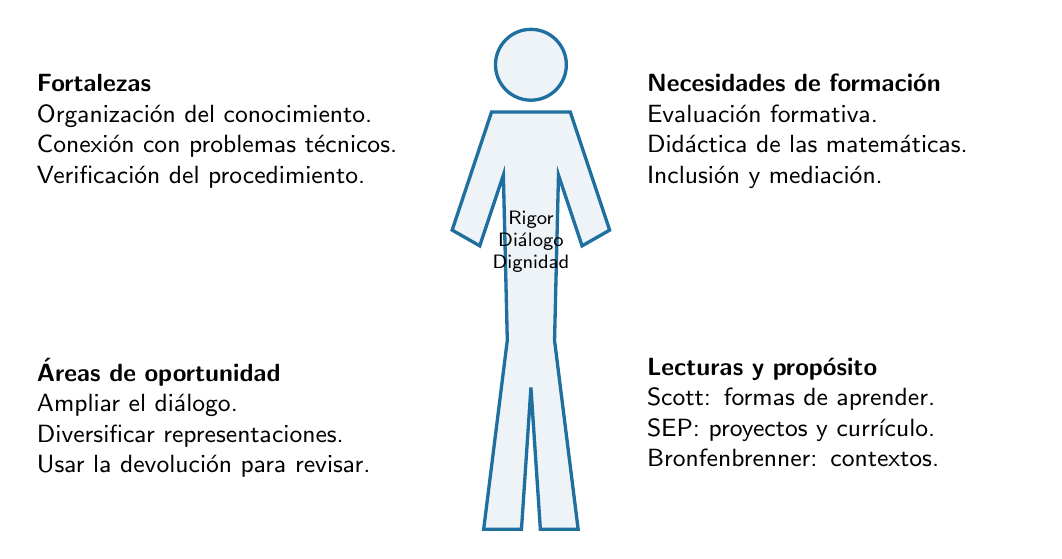
\begin{tikzpicture}[x=1cm,y=1cm,every node/.style={font=\small},shorten >=2pt]
\draw[iiiepeBlue,very thick,fill=iiiepeBlue!8] (0,3.7) circle (.45);
\draw[iiiepeBlue,very thick,fill=iiiepeBlue!8] (-.5,3.1)--(-1,1.6)--(-.65,1.4)--(-.35,2.3)--(-.30,.2)--(-.6,-2.2)--(-.12,-2.2)--(0,-.4)--(.12,-2.2)--(.6,-2.2)--(.30,.2)--(.35,2.3)--(.65,1.4)--(1,1.6)--(.5,3.1)--cycle;
\node[align=center,text width=1.25cm,font=\scriptsize] at (0,1.45){Rigor\\Diálogo\\Dignidad};
\node[anchor=north east,align=left,text width=4.8cm] at (-1.35,3.7){\textbf{Fortalezas}\\Organización del conocimiento.\\Conexión con problemas técnicos.\\Verificación del procedimiento.};
\node[anchor=north east,align=left,text width=4.8cm] at (-1.35,.1){\textbf{Áreas de oportunidad}\\Ampliar el diálogo.\\Diversificar representaciones.\\Usar la devolución para revisar.};
\node[anchor=north west,align=left,text width=4.8cm] at (1.35,3.7){\textbf{Necesidades de formación}\\Evaluación formativa.\\Didáctica de las matemáticas.\\Inclusión y mediación.};
\node[anchor=north west,align=left,text width=4.8cm] at (1.35,.1){\textbf{Lecturas y propósito}\\Scott: formas de aprender.\\SEP: proyectos y currículo.\\Bronfenbrenner: contextos.};
\end{tikzpicture}\end{center}
\section{Fortalezas y áreas de oportunidad}
La organización del conocimiento es una fortaleza de mi trayectoria: me permite establecer objetivos, secuencias y relaciones entre conceptos y trabajo. En mantenimiento y mecatrónica, esa mirada puede traducirse en problemas con variables identificables, procedimientos verificables y criterios claros. No doy por probado un efecto sobre el aprendizaje; reconozco un recurso profesional que puedo poner al servicio de la enseñanza.
La vinculación con ingeniería ofrece contextos para discutir modelación, unidades, incertidumbre y decisiones. También exige revisar un límite: un contexto industrial no resulta significativo automáticamente para todos. Debo explorar qué conocen los estudiantes y permitirles formular preguntas, en lugar de suponer que el interés por la aplicación técnica es compartido.
Mi principal área de oportunidad es superar una enseñanza excesivamente mecánica. Explicar con claridad y pedir ejecución puede dejar fuera los motivos del error, las interpretaciones y las condiciones personales. Quiero ampliar los espacios de diálogo y las representaciones, conservar primeras respuestas y permitir revisiones. Estas son metas de desarrollo, no prácticas cuya frecuencia o eficacia ya haya medido.
\section{Necesidades de formación y bibliografía}
Necesito profundizar en evaluación formativa para convertir la información de las tareas en decisiones de apoyo. Una rúbrica no basta si termina en una nota: debe orientar una corrección que el estudiante pueda utilizar. También busco herramientas de didáctica de las matemáticas para distinguir dificultad conceptual, representacional y operativa.
Scott (2015a, 2015b) me ofrece un marco para revisar aprendizajes y demandas del contexto; las propuestas de la SEP (2022a, 2022b) ayudan a diseñar problemas y proyectos con participación; Bronfenbrenner (1987) permite examinar relaciones entre aula, institución, familia y contexto social. No utilizaría estas lecturas como etiquetas, sino como preguntas para analizar decisiones concretas.
\section{Decisiones que concretan mi desarrollo profesional}
En mantenimiento y mecatrónica, un procedimiento debe ser seguro, trazable y verificable; en ingeniería, además debe justificarse el modelo. Esa base constituye una fortaleza de mi formación. El cambio humanista no consiste en abandonar el rigor, sino en revisar cómo organizo el acceso a él: qué sabe cada estudiante, cómo interpreta el problema y qué oportunidades tiene de explicar una decisión.
Para trabajar el área de oportunidad identificada, propongo sustituir una parte de la demostración inicial por una predicción individual y una discusión breve de estrategias. Después conservaría la explicación técnica necesaria, pediría aplicar el procedimiento y utilizaría una devolución para producir una segunda versión. La comparación entre ambas explicaciones permitiría examinar qué cambió, en lugar de inferir comprensión por la entrega del producto.
La formación que busco debe ayudarme a distinguir una dificultad de lenguaje, una dificultad matemática y una barrera de acceso. Ante la misma respuesta incompleta, las decisiones pueden ser diferentes: reconstruir una unidad, ofrecer un apoyo visual o ajustar la forma de participación. Mi identidad docente se fortalece cuando esas decisiones tienen razones y se revisan con evidencia.

\section{Compromiso de desarrollo}
Propongo trabajar una secuencia en la que cada estudiante formule una predicción, explique un procedimiento y utilice una devolución para revisarlo. Compararía la respuesta inicial con la final y anotaría qué apoyo fue necesario. La meta es integrar el rigor que caracteriza mi formación industrial con una enseñanza que reconozca a las personas y les permita construir autonomía.

\section{Formación técnica y responsabilidad educativa}
El perfil de Mecatrónica del CONALEP (2025, pp. 1--3) vincula formación integral y juicio ético con diagnóstico, medición y mantenimiento. Esa referencia respalda la pertinencia de relacionar rigor técnico y atención a la persona. En mi perfil docente, la aplicación consiste en pedir razones y decisiones justificadas, con oportunidades de participación y revisión; no en reducir la enseñanza al cumplimiento de una operación.
\needspace{5\baselineskip}\section*{Referencias}
{\setstretch{1.15}\setlength{\parskip}{6pt}
\par\hangindent=1.27cm\hangafter=1  Bronfenbrenner, U. (1987). \textit{La ecología del desarrollo humano}. Paidós.
\par\hangindent=1.27cm Colegio Nacional de Educación Profesional Técnica. (2025). \textit{Perfil de egreso: Profesional Técnico-Bachiller en Mecatrónica. Modelo Académico 2025}. Secretaría Académica. \url{https://www.conalep.edu.mx/sites/default/files/micrositios/perfil_egreso_2025/ElectyElectro/PE25_Mecatr%C3%B3nica.pdf}
\par\hangindent=1.27cm\hangafter=1  Scott, C. L. (2015a). \textit{El futuro del aprendizaje 1: ¿Por qué deben cambiar el contenido y los métodos de aprendizaje en el siglo XXI?} (Investigación y prospectiva en educación, 13). UNESCO.
\par\hangindent=1.27cm\hangafter=1  Scott, C. L. (2015b). \textit{El futuro del aprendizaje 2: ¿Qué tipo de aprendizaje se necesita en el siglo XXI?} (Investigación y prospectiva en educación, 14). UNESCO.
\par\hangindent=1.27cm\hangafter=1  Secretaría de Educación Pública. (2022a). \textit{Plan de Estudio para la educación preescolar, primaria y secundaria}. SEP.
\par\hangindent=1.27cm\hangafter=1  Secretaría de Educación Pública. (2022b). \textit{Sugerencias metodológicas para el desarrollo de los proyectos educativos} [Extracto de \textit{Avance del contenido para el libro del docente. Primer grado}, material en proceso de edición, pp. 64--82, 23--24]. SEP.
}

\end{document}
